\subsection{Comportamiento Esperado de PageRank}
\label{subsec:exp1}
\begin{LaTeXdescription}
    \item[Objetivo] Ejemplificar el comportamiendo esperado de pagerank.
        Proponemos, a su vez, que el orden obtenido por PageRank ser\'a el mismo
        para cualquier factor de navegaci\'on $\alpha$\footnote{Lo llamamos
        ''factor de navegaci\'on'' al par\'ametro $\alpha$ ya que el mismo
        determina el peso/importancia del grafo/matriz de navegaci\'on $S$
        (definida en la ecuaci\'on \ref{eq:S}, p\'agina \pageref{eq:S}). Se
        puede observar en la definici\'on de $M$ en la p\'agina
        \pageref{eq:M_def} que justamente $\alpha$ define en que porporci\'on
        estar\'an inclu\'idos en $S$ y la matriz de teletransportaic\'on
        uniforme. Llamamos entonces a $\alpha$ factor de navegaci\'on, ya
        que de alguna manera nos indica directamente sin tener que pensar en
        $(1-\alpha)$ en que proporci\'on participa $S$ en $M$, y decimos que
        $S$ es una matriz de navegaci\'on ya que es la matriz que contiene
        los datos de la matriz de conectividad con el inconveniente de los
        dangling nodes resuelto.}, aunque las probabilidades del vector
        resultado (asociadas a cada nodo) cambiar\'an seg\'un este par\'ametro.

    \item[Proposici\'on] No creemos que haga falta aclarar mucho. Ya se present\'o y explic\'o
        m\'etodo a utilizar. Generaremos un grafo de entrada lo suficientemente
        peque\~no que nos permita calcular a mano el resultado de PageRank y
        explicar el porque de su resultado en base al conocimiento del m\'etodo.

    \item[M\'etodo de Experimentaci\'on] Realizamos la b\'usqueda en
        ''site:uba.ar'' \emph{Google}\cite{google} y tomamos los primeros 10
        resultados.  Generamos una instancia de entrada utilizando las
        herramientas de la c\'atedra y estos 10 resultados. Por \'ultimo, dada
        esta instancia de prueba, calculamos el \emph{ranking} con el m\'etodo
        PageRank para varios distintos factores de navegaci\'on $\alpha$.

    \item[Resultados, an\'alisis y discusi\'on]
\end{LaTeXdescription}

\begin{figure}
    \centering
    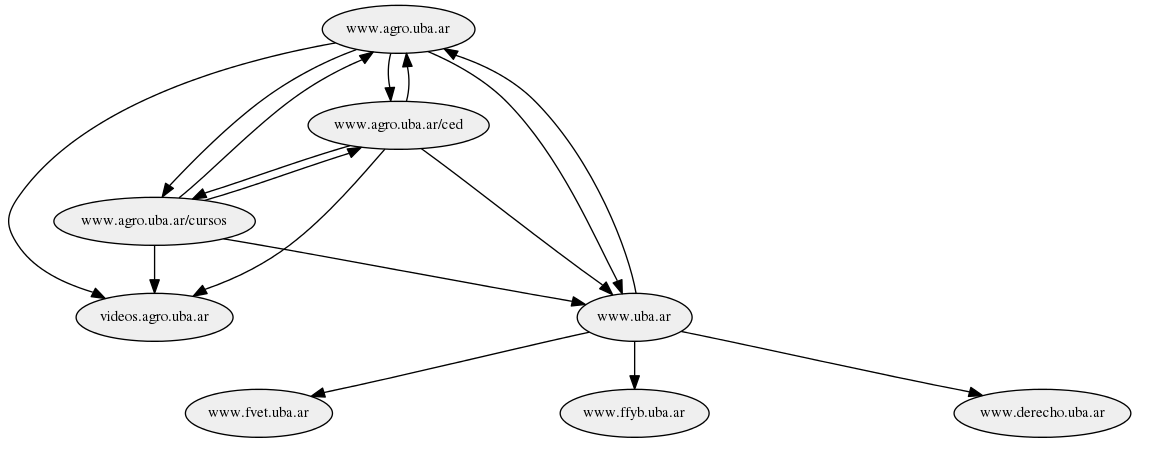
\includegraphics[width=\textwidth]{exp1_conn_graph.png}
    \caption{Grafo de conectividad de la instancia generada con los links
        obtenidos mediante la b\'usqueda en \emph{Google}}
    \label{fig:uba.ar_graph}
\end{figure}

\begin{table}
    \centering
    \caption{\'Ordenes obtenidos y sus porcentajes para los resultados obtenidos
        de la b\'usqueda ''site:uba.ar'' en \emph{Google}}
    \setlength{\tabcolsep}{3pt}
    \begin{tabular}{|l||r||l||r|r|r|r|r|r|r|r|r|}
        \hline\hline
        \multicolumn{2}{|c||}{Caso particular $\alpha = 0$}&
        \multicolumn{10}{c|}{Casos $0 < \alpha < 1$}\\
        \hline
        Orden/P\'agina & 0 & Orden/P\'agina & 0.1&0.2&0.3&0.4&0.5&0.6&0.7&0.8&0.9\\
        \hline\hline
        derecho.uba.ar& 0.1& 
        videos.agro.uba.ar& 0.0984973& 0.0969883& 0.0954716& 0.0939457&
        0.0924093& 0.0908605& 0.0892978& 0.0877193& 0.0861231\\
        %
        orga2.exp.dc.uba.ar& 0.1&
        uba.ar& 0.0959086& 0.0916284& 0.0871502& 0.0824635& 0.0775579&
        0.0724212& 0.0670411& 0.0614038& 0.0554939\\
        %
        agro.uba.ar& 0.1&
        agro.uba.ar& 0.103548& 0.107198 & 0.110953 & 0.114823 & 0.118812 &
        0.122929 & 0.127182 & 0.131579 & 0.13613\\
        %
        ffyb.uba.ar& 0.1&
        agro.uba.ar/cursos& 0.0984973& 0.0969883& 0.0954716& 0.0939457
        & 0.0924093& 0.0908605& 0.0892978& 0.0877193& 0.0861231\\
        %
        uba.ar& 0.1&
        agro.uba.ar/ced& 0.103548& 0.107198 & 0.110953 & 0.114823
        & 0.118812 & 0.122929 & 0.127182 & 0.131579 & 0.13613\\
        %
        fvet.uba.ar& 0.1&
        fvet.uba.ar& 0.0984973& 0.0969883& 0.0954716& 0.0939457
        & 0.0924093& 0.0908605& 0.0892978& 0.0877193& 0.0861231\\
        %
        videos.agro.uba.ar& 0.1&
        ffyb.uba.ar& 0.103548& 0.107198 & 0.110953 & 0.114823 & 0.118812
        & 0.122929 & 0.127182 & 0.131579 & 0.13613\\
        %
        iigg.sociales.uba.ar& 0.1&
        derecho.uba.ar& 0.0959086& 0.0916284& 0.0871502& 0.0824635
        & 0.0775579& 0.0724212& 0.0670411& 0.0614038& 0.0554939\\
        %
        agro.uba.ar/cursos& 0.1&
        iigg.sociales.uba.ar& 0.101023& 0.102093 & 0.103212 & 0.104384
        & 0.105611 & 0.106895 & 0.10824& 0.109649 & 0.111127\\
        %
        agro.uba.ar/ced& 0.1&
        orga2.exp.dc.uba.ar& 0.101023& 0.102093 & 0.103212 & 0.104384
        & 0.105611 & 0.106895 & 0.10824& 0.109649 & 0.111127\\
        %
        \hline
        Probabilidad Total& 1&
        Probabilidad Total& 0.9999991& 1.0000017& 0.9999982& 1.0000011&
        1.0000017& 1.0000009& 1.0000016& 1.0000005& 1.0000011\\
        \hline\hline
    \end{tabular}
\end{table}
